\clearpage
\section{Umsetzung Benchmark}\label{sec:ZigbeeUmsetzungBenchmark}
\todo[inline]{Komplette Beschreibung der Firmware unterteilt in die 3 Nodetypen. Besonderheiten herausstreichen und allfällige Schwierigkeiten aufzeigen.}

\subsection{Benchmark und Stack Parameter}\label{subsec:BenchmarkundStackParameter}


\begin{table}[h]
\centering
\begin{adjustbox}{width=1\textwidth}
\begin{tabular}{lll}
Stack Init Time & 60000 ms & \begin{tabular}[t]{@{}l@{}}Zeit die benötigt wird um den Stack für den Benchmark\\zu initialisieren. Das Zigbee Netzwerk benötigt eine\\gewisse Zeit um sich aufzubauen\end{tabular} \\
IEEE Channel & 15 & Zigbee Kanal der verwendet wird um das Mesh aufzubauen. \\
Client Endpoint & 1 & Nummer für den Client Endpoint im ZCL Level Cluster \\
Server Endpoint & 10 & Nummer für den Server Endpoint im ZCL Level Cluster \\
Group ID & 0xB331 & \begin{tabular}[t]{@{}l@{}}Default Group ID. Zu diesem Wert wird der Index für die\\zugewiesene Gruppe addiert um die\\Gruppenzugehörigkeit festzulegen.\end{tabular}
\end{tabular}
\end{adjustbox}
\caption{Messgrössen Gewinnung und Verwendung}
\label{tab:MessgrössenGewinnungundVerwendung}
\end{table}


\subsection{Benchmark Message}\label{subsec:BenchmarkMessage}

\subsection{Zigbee Stack Implementation}\label{subsec:ZigbeeStackImplementation}

\subsubsection{Topologie}\label{subsubsec:ZigbeeTopologie}

Mesh mit 50 ZR (Zigbee Router)


\subsubsection{Funkkanal Wahl im 2.4GHz ISM Band}\label{subsubsec:FunkkanalWahlim2.4GHzISMBand}

\begin{figure}[h]
	\centering
	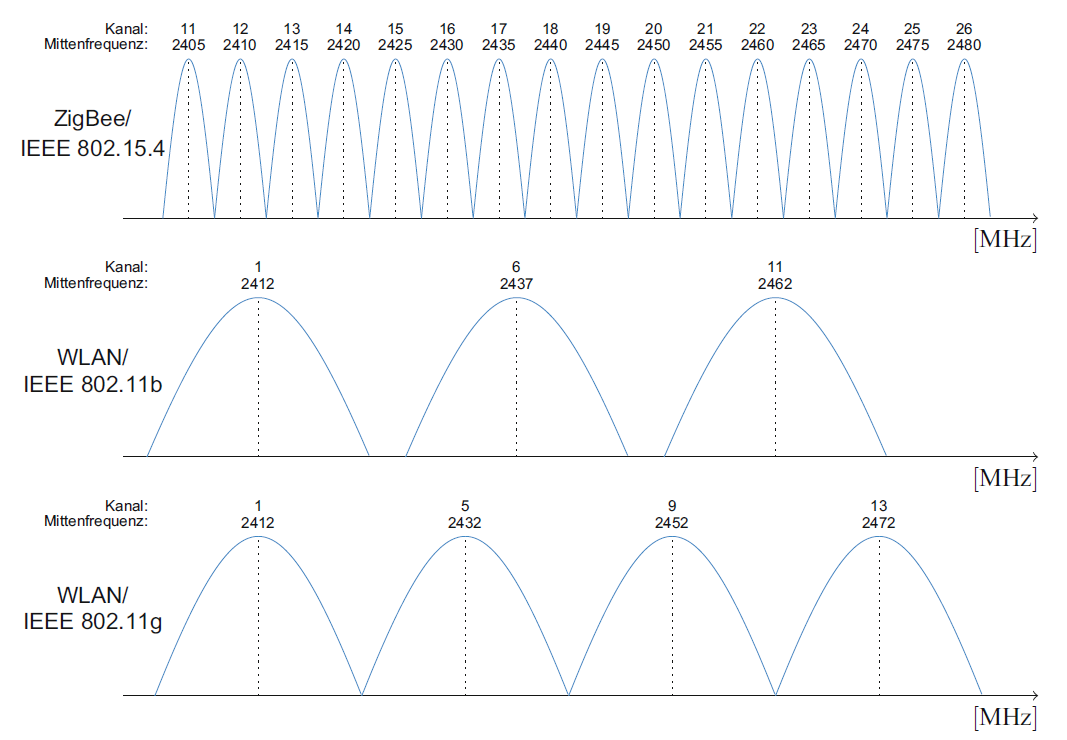
\includegraphics[width=0.8\textwidth]{Funkkanaele_Konkurrenz_IEEE.png}
	\caption{Konkurrenz IEEE und WLAN Funkkanäle \cite{markus_krause_rainer_konrad_drahtlose_2014}}
	\label{fig:KonkurrenzIEEEundWLANFunkkanäle}
\end{figure}

\subsubsection{ZCL Level Cluster}\label{subsubsec:ZCLLevelCluster}

\subsubsection{Endpoint Handler}\label{subsubsec:EndpointHandler}

Costum Endpoint Handler: ZBAFSETENDPOINTHANDLER anstatt Standard ZCL Device Callback

\subsubsection{APS Header}\label{subsubsec:Header}


\begin{figure}[h]
	\centering
	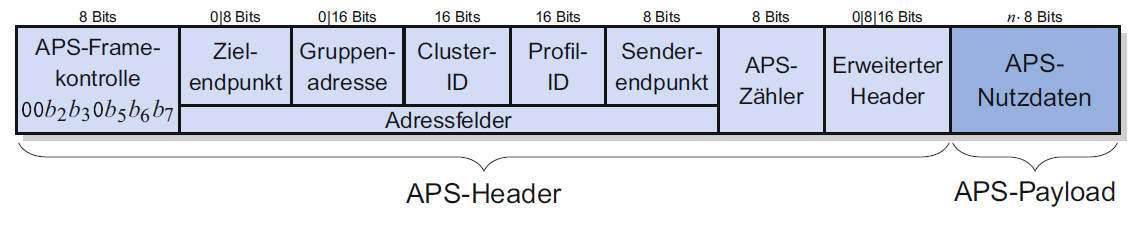
\includegraphics[width=0.8\textwidth]{Zigbee_APS_Datenframe.png}
	\caption{Aufbau APS Datenframe \cite{markus_krause_rainer_konrad_drahtlose_2014}}
	\label{fig:KonkurrenzIEEEundWLANFunkkanäle}
\end{figure}


\subsubsection{Adressierung}\label{subsubsec:Adressierung}

